\documentclass[a4paper]{article}

\usepackage[english]{babel}
\usepackage[utf8]{inputenc}
\usepackage[hidelinks]{hyperref}

\usepackage{graphicx}
\graphicspath{ {images/} }

\usepackage{setspace}
\usepackage{pdfpages}
\usepackage{xspace} %Removes space after commands
\usepackage{fancyhdr}
\usepackage{lastpage}
\usepackage{verbatim}
\usepackage{url}

%%% BibTeX %%%
\usepackage{cite}
% JS function to get BibTeX entry from WebAssembly website
\begin{comment}
function BibTeX() {
	let subject = document.title.replace(/ - WebAssembly/, '').replace(' ', '-').toLowerCase();
    return `@misc{website:wasm-${subject},
	author = "The WebAssembly working group",
	title = {{${document.title}}},
	howpublished = "${document.URL}",
	note = {Online; accessed 13 May 2017},
}`;
}
\end{comment}

% source: https://tex.stackexchange.com/a/35044
\makeatletter
\newcommand\footnoteref[1]{\protected@xdef\@thefnmark{\ref{#1}}\@footnotemark}
\makeatother

\makeatletter
\renewcommand\listoffigures{%
        \@starttoc{lof}%
}
\makeatother

% Code highlighting
\usepackage{minted}
% Highlight theme
\usemintedstyle{trac}

\pagestyle{fancy}
\fancyhf{}

\lfoot{Page \thepage \hspace{1pt} of \pageref{LastPage}}

\usepackage[margin=0.8in]{geometry}

\title{Bachelor Project Report: Compiling MicroC to WebAssembly}

\begin{document}
%\pagenumbering{gobble} %Remove page numbers
\begin{titlepage}
	\centering
	{\scshape\LARGE IT University of Copenhagen \par}
	\vspace{1cm}
	{\scshape\Large Bachelor Project Report\par}
	\vspace{1.5cm}
	{\huge\bfseries Compiling MicroC to WebAssembly \par}
	\vspace{2cm}
	{
\includegraphics{WebAssemblyLogo} \par}
	\vspace{2cm}
	{\Large\itshape Andreas Bjørn Hassing Nielsen\par}
	abhn@itu.dk\\
	\vspace{2cm}
	{\Large Abstract\par}
	%TODO: Write an awesome abstract.
	{\bfseries This is where the abstract will go.}
	\vfill
% Bottom of the page
	{\large \today\par}
\end{titlepage}
\newpage

\tableofcontents

\newpage
\section{Introduction}
\label{sec:introduction}
The purpose of this project is to build a compiler, also called a translator, from MicroC to WebAssembly, using FsLexYacc\footnote{\label{footnote:fslexyacc-url}http://fsprojects.github.io/FsLexYacc/} and F\#\footnote{http://fsharp.org/}. The learning goals are to develop an understanding of WebAssembly, and to improve my knowledge of compiler design.

MicroC is a C-like language described by Peter Sestoft in the book Programming Language Concepts~\cite{PLC}. The original lexer and parser code can be found at his website\footnote{http://www.itu.dk/people/sestoft/plc/}.\\

This report will give a more in-depth explanation of how the WebAssembly format works, and discuss how a compiler, that goes from a C-like language to this new platform, can be designed.\\

I have previously had experience with compiler design. In the course: "Programs as Data", I extended the MicroC compiler with a handful of features: optimisations in the backwards continuation-based MicroC compiler, more looping constructs, compound assignment operators, increment/decrement operators and more.

While these alterations don't explicitly teach compiler design from-scratch, I had confidence that observing and analysing the behaviour of the pre-defined compiler yielded enough knowledge to get started writing my own.

MicroWac, the name of the MicroC to WebAssembly compiler described in this report, uses the abstract syntax (with some extensions) and the lexer and parser from the original MicroC project by Peter Sestoft. The compiler is written from scratch, as the differences between the MicroC stack machine and WebAssembly binaries are significant.

\section{Background and Problem Definition}
\label{sec:problem-definition}
WebAssembly (WASM) is a new up-and-coming binary code format for the user-facing web, designed to work alongside JavaScript as a more portable, size- and load-time-efficient, ahead-of-time-compiled alternative. 

The binary WASM format is not bound to be emitted by JavaScript (asm.js) only, potentially bringing your favourite language to the browser front-end. If a language can compile to a intermediate representation supported by WASM (LLVM IR, for instance), it can be compiled to the binary WASM format. 

The purpose of this project is to shed some light on the unfinished WebAssembly specification. To assist in meeting this goal, a compiler will be designed, that compiles from a simple programming language, MicroC, to a WASM format that can be run in a WASM-enabled browser today (currently requiring Firefox Nightly or Chrome Canary with WASM flags set to enabled\footnote{At the time of writing (May, 2017), setting flags or using a nightly browser version is no longer required. Major browsers now support WASM out of the box: https://lists.w3.org/Archives/Public/public-webassembly/2017Feb/0002.html}).

\subsection{Method}
\label{sec:problem-definition:method}
What follows is the planned activities and sources of information.
\begin{itemize}
	\item Translation of MicroC to the binary WebAssembly format, using FsLexYacc\footnoteref{footnote:fslexyacc-url}, as used in the Programs as Data course (fall 2016).
	\item Course books from Programs as Data (fall 2016) will be used as knowledge base for MicroC to WebAssembly translation:
		\begin{itemize}
			\item Peter Sestoft: Programming Language Concepts. Springer 2012.
			\item Torben Mogensen: Basics of Compiler Design. DIKU 2010. Chapters 2 and 3.
		\end{itemize}
	\item Knowledge of WebAssembly will be gained through the official website (http://webassembly.org/) and links branching out from it.
	\item Creation of prototype: web interface that lets users type MicroC in a window, and see it generate WebAssembly in some human-readable format, either s-expression or linear bytecode. The prototype will also give users the ability to run their code as WebAssembly, given that the browser in use supports it.
	\item Reflection over, either the security behind WebAssembly or the portability of it between browsers and platforms.
\end{itemize}

\noindent If time allows:
\begin{itemize}
	\item Extensions to the MicroC language will be implemented.
	\item Simple optimizations to the generated WebAssembly code.
\end{itemize}

\subsection{Changes to Method and Problem Definition}
\label{sec:problem-definition:changes}
I realized while coding the compiler that I would have to stop working on it prematurely to get the web back- and frontend working as well. This was an underestimation on my part.

In a meeting with Niels Hallenberg on May 1st we agreed to discard the web part of this project. To make up for the loss I have added a flag (\texttt{-html}) to the compiler which generates a HTML template to go along with the \texttt{.wasm} output. The HTML template makes it easy to test compiled WebAssembly binaries, as you can serve the HTML with a simple HTTP server, see section~\ref{sec:peripherals:testing-wasm},~\nameref{sec:peripherals:testing-wasm}, on how to do that.\\

\noindent I do not feel that I have the knowledge required to reflect over the security of WebAssembly. Discussing the portability of WebAssembly also feels a little out of my reach - I can make assumptions about how I fear that later versions of WebAssembly will diverge, in the case that some browser vendors feel that development of the standard is too slow, but in the end I do not feel that this is a very important discussion to have. Instead I have spent some time extending MicroC with \texttt{import} and \texttt{export} keywords, and discuss the implementation of these in section~\ref{sec:technical},~\nameref{sec:technical}.\\

\noindent It is no longer required to set flags in browsers, or use nightly versions in order to run WebAssembly modules.

\newpage
\section{Problem Analysis}
\label{sec:problem-analysis}
In this section, the problem will be dissected and analysed. The definition of a compiler and a stack machine is discussed, and the WebAssembly specification and binary encoding is scrutinised. Some history is also supplied, to help explain the purpose and origin of WebAssembly.

\subsection{Compilers in General}
\label{sec:problem-analysis:compilers}
Before designing a compiler, an important question must be put forth and answered: "What is a compiler?".

According to the definition laid out by Mogensen~\cite{BCD}, a compiler is a program that takes the source code of another program as input, usually some higher-level language such as C\#, and compiles it to a lower-level representation, Common Intermediate Language code - in the case of C\#, or binary machine code instructions - in the case of C. There are more low-level representations out in the wild, but these two will be the ones referenced to in this report.

Compilers are separated into a frontend and a backend. The frontend is responsible for parsing the code written by a developer and turning it into an abstract syntax. The backend converts the abstract syntax into a format the targeted system can understand. In MicroC, the lexer and parser that are defined in \texttt{CLex.fsl} and \texttt{CPar.fsy} respectively, make up the frontend part of the compiler, whereas \texttt{WasmMachine.fs} and \texttt{Wasmcomp.fs} make up the backend part. Together, the frontend and backend work in tandem to take user-written code as input, and output a program that the machine can run.

The decoupling of the frontend and backend in a compiler yields a great benefit: A new frontend can be added for a backend, thus supporting more languages that compile to the same type of backend, and a new backend can be added to a frontend, such that the compiler supports more systems. If, for instance, we wrote a compiler that compiles from F\# to WebAssembly, we could add an extra frontend that took care of C\# and reuse the backend. This separation is used nicely in the LLVM compiler, which supports many backends and frontends, and defining a target-independent optimiser which can be used across languages and systems\footnote{http://llvm.org/}.\\

Many programs are written in higher-level languages that run within an assisting runtime environment and compiles to a variant of bytecode, with an instruction set specified in the virtual machine of the runtime. When the runtime is started and the program bytecode is passed to it, it performs a just-in-time (JIT) compilation to native machine code using the instruction set of the machine's processor. .NETs' CLR and Javas' JRE are two such runtimes that both support several higher-level languages, such as C\#, F\#, Java and Scala. Runtime environments often come equipped with integrated memory management in the form of a garbage collector.

Programs written in comparatively lower-level languages, such as C and C++, are usually compiled ahead-of-time (AOT) to native machine code using the instruction set of the compiling machine. One can often configure the compiler to target other operating systems and processor architectures than that of the compiling system. In these lower-level languages, the developer is often challenged with manually managing dynamic memory. In C, this means using \texttt{malloc} and \texttt{free} for allocation and deallocation of memory while the program is running.

Note, that nothing stops us from implementing a runtime environment that supports a language which is usually AOT compiled, such as C. Such a runtime environment can then execute code written in that language as a JIT compiled application. With C, this task is most likely non-trivial.\\

The notion of forward and backward compilation will be mentioned in this report, it describes the direction of compilation. Peter Sestoft has designed a forward compiler for MicroC (\texttt{Comp.fs}) and a backward continuation based compiler (\texttt{ContComp.fs}. The purpose of the backward continuation compiler is to display how some easy optimisations can be implemented when compiling in that particular direction. MicroWac will be a forward compiler with no optimisations.

\subsubsection{Benefits of AOT- over JIT Compilation}
\label{sec:problem-analysis:benefits-of-aot}
\textbf{Type Safety} When a statically typed language is compiled ahead-of-time, the compiler can complain to the developer before the program hits runtime. For instance, if the developer attempts to assign a char value to a variable that is declared to contain an integer, the compilation will fail. This is useful for producing correct code. JavaScript is a loosely typed language, meaning that type checking occurs at runtime, and type errors that the developer was not notified of during development will show up in the browser.\\

\noindent \textbf{Optimisations} While optimisations can be made by both an AOT and JIT compiler, an AOT has all the time a developer has to spare to optimise. A JIT will need to weigh the potential gain of an optimisation against slowing down the program during the consideration process. This makes an AOT compiler preferred for live and runtime critical systems - as execution is deterministic.

\subsection{Stack Machines}
Stack machines implement some derived behaviour of what is known as the abstract stack machine. The stack machine executes code by pushing values onto- and popping values off a stack data structure, hence the name. The instructions are added to the stack using reverse polish notation, also called postfix notation. This notation works by turning infix operators into postfix, for instance: \mintinline{fsharp}{3 + 4} becomes \mintinline{fsharp}{3 4 (+)}. The machine keeps popping the top element on the stack to figure out what to do next.

Specific implementations of stack machines have a set of instruction codes that can be used. For instance, the WebAssembly stack machine has the \texttt{i32.add} instruction code, which, when popped, pops two operand values off the stack, adds them together and pushes the result back onto the stack. Several arithmetic-, logic- and other instruction codes are available in the WebAssembly stack machine~\cite{website:wasm-binary-encoding}.

Most computers aren't pure stack machines, but some derived combination of a stack machine, a register machine (which uses registers to store operands and intermediate values) and possibly other machine types. As such, a stack machine can be thought of as an abstraction on top of the machine architecture.

Assembly language (not WebAssembly) is the closest, somewhat sane, code representation we have to code directly against the central processing unit. This language uses reverse polish notation, just like a stack machine, and utilises registers that are closer to the central processing unit than random access memory. When a browser compiles WebAssembly (which does not use registers), registers are used, and disassembling the LLVM output of a WebAssembly compilation done by browsers\footnote{The tool that enables this level of inspection: https://mbebenita.github.io/WasmExplorer/} proves this\footnote{WasmExplorer used to compile a simple C program to WebAssembly, then to LLVM x86 Assembly: https://goo.gl/nUqTZ1}.

A specific version of the Assembly language exists for each instruction set architecture, but they usually have several similarities. An Assembly language exists which attempt to support several platforms\footnote{NASM (The Netwide Assembler) is an assembly language that is designed for portability, and can be compiled for execution on multiple operating systems and processor architectures (x86/x86-64): http://www.nasm.us/}.

%TODO: add more to AOT benefits?
%TODO: add JIT benefits?
\newpage
\subsection{History of Web Coding}
\label{sec:problem-analysis:history}
Less than a year ago there was only 1 language that could run natively in all browsers: JavaScript. The web is built around it, and the language has flourished and expanded beyond the land of browsers, in the form of execution environments such as Node.js\footnote{https://nodejs.org/} and native application frameworks such as React Native\footnote{https://facebook.github.io/react-native/} and Electron\footnote{https://electron.atom.io/}.

Attempts have been made to make JavaScript run faster, but ultimately no standards other than WebAssembly caught on. One of the more popular attempts is asm.js\footnote{http://asmjs.org/spec/latest/}. asm.js is a subset of JavaScript, with tooling that allows for source-to-source compilation from languages such as C and C++ to asm.js. The subset allows static type checking by browsers that implement a specific parser for asm.js. Drafted in 2014 - asm.js yielded good results\footnote{http://asmjs.org/faq.html}, but work on the format seems to have shifted to WebAssembly, due to the large size of compiled code bases (non-binary). The binary WebAssembly format is much smaller, and can be compressed even more than the code yielded by asm.js, furthermore parsing of binary data is significantly faster than that of strings, thus decreasing the time-to-execution of compiled WebAssembly modules versus asm.js code.

\subsubsection{JavaScript}
JavaScript is a loosely typed language that runs in browsers. The JavaScript code created by a software developer needs to be sent via a server to the visitors browser, the code will then execute immediately.

JavaScript is compiled by a JIT compiler at runtime\footnote{This is not always true. Ignition, a newly developed interpreter for V8 (Chrome's JavaScript engine), is used alone or along with JIT compilation, especially on devices where a lower- memory footprint, or battery usage is preferred over high performance (Smartphones, for instance)~\cite{video:thompson-js-perf-v8-and-wasm}.}, which takes the code, converts it into abstract syntax and then to machine code~\cite[p.~13]{slides:lund-v8}. During the execution of a JavaScript program, the JIT compiler will attempt to optimise the generated machine code by making probabilistic assumptions about program behaviour. These assumptions can eventually fail, thus forcing the JIT to throw away optimisations based on falsified claims - this is a cause of non-deterministic execution speed of JavaScript programs. The JIT's that are found in modern browsers make a lot of intelligent optimisations on what is generally referred to as \texttt{warm} and \texttt{hot} code paths\footnote{Warm and hot code describes code paths that are executed regularly and often, respectively.}, thereby greatly increasing performance without sacrificing excessive resources. When a JIT compiler is run on a system with multiple processor cores, it can run in parallel, thereby generating optimisations without blocking the main thread of the browser.

\subsection{WebAssembly}
\label{sec:problem-analysis:webassembly}
WebAssembly can be expressed using two formats: a binary syntax that can be executed in browsers (and Node.js behind a flag: \texttt{--expose-wasm}), and a textual representation called the S-expression syntax.

The binary syntax contains a magic number which states that the module is WebAssembly and the version number of the binary. Then follows a number of sections that describe the intricacies of the module. The binary module is described in more detail in section~\ref{sec:problem-analysis:webassembly:binary},~\nameref{sec:problem-analysis:webassembly:binary}.

Binary files are not readable to the human eye, so S-expressions is also available. The S-expression syntax for WebAssembly was described in order to keep the "View Source" functionality of the Web\footnote{You can view the source code of any JavaScript code running in your browser by right-clicking a website. The WebAssembly working group wishes to keep this tradition with WebAssembly~\cite{website:wasm-webassembly-high-level-goals}.}.

The WebAssembly Working group has developed WABT\footnote{https://github.com/WebAssembly/wabt/} (WebAssembly Binary Toolkit), a toolkit that allows bidirectional translation between the binary syntax and the S-expression syntax. Browsers could use this toolkit, or a functionally equivalent derivative, to translate binaries to the S-expression syntax, such that viewing the source of WebAssembly binaries on arbitrary websites is easy.

WebAssembly is designed to work well together with JavaScript~\cite{website:wasm-webassembly-high-level-goals}. This can be deduced without looking at the goals of WebAssembly, by inspecting the design of the binary- and textual representation of WebAssembly. Code compiled to WASM is turned into modules that can be instantiated from JavaScript, and WebAssembly modules can selectively define which components to expose to- and import from JavaScript.

Exported and imported components from and to WASM can be of types: functions, variables and memory segments. This design allows WASM modules to make use of dependency injections, which can assist in decoupling code and separating implementation concerns.

\subsubsection{The S-expression Syntax}
\label{sec:problem-analysis:webassembly:s-exp}
The S-expression syntax is easily explained with an example:
\begin{minted}[tabsize=2]{javascript}
(module
  (func $printi (import "imports" "printi") (param i32))
  (func $start
    (local i32)
    i32.const 5
    i32.const 3
    i32.add
    set_local 0
    get_local 0
    call $printi
  )
  (start $start)
)
\end{minted}
The code above describes a module. Within that module are functions \texttt{printi} and \texttt{start}. The \texttt{printi} function is imported from an object named \texttt{imports} and a field within that object named \texttt{printi}, it takes a single 32-bit integer as parameter. The \texttt{start} function declares a local 32-bit integer variable. Note that local variables need to be declared at the top of a function, this behaviour is even more strict than the C89 specification, which allows variable declarations in the top of any block. The function then pushes constant 32-bit integers $5$ and $3$ onto the stack, and then a 32-bit addition operator. The local variable is set to the top value on the stack (the result of the addition) and \texttt{printi} is called, taking the top value on the stack as argument.

A \texttt{start} component dictates which function will run at instantiation-time. Functions must not take any arguments and must not return a value in order to be valid for \texttt{start}. This is in contrast to the typical \texttt{main} entry point function, which usually takes an argument count and a string array of arguments. MicroC uses the \texttt{main} version, so a compromise must be thought up to allow running MicroC programs at instantiation-time.

The \texttt{printi} function needs to be injected into the module from within the browser. This yields a freedom to the developer, offering the opportunity to easily change behaviour of WebAssembly modules. For instance, if a WebAssembly module imports some logging function, the developer can hand the module a very verbose logging function in the development environment, and a more quiet logging function in the released environment.

\subsubsection{The Binary Format}
\label{sec:problem-analysis:webassembly:binary}
The binary format of WebAssembly modules contains the magic number and several sections that determine the behaviour of the modules.

The S-expression syntax example from section~\ref{sec:problem-analysis:webassembly:s-exp},~\nameref{sec:problem-analysis:webassembly:s-exp} has been compiled to binary format and explained in detail. This binary analysis can be found in~\ref{sec:appendix:wasm-examples:binary-print},~\nameref{sec:appendix:wasm-examples:binary-print}.

\subsubsection{Linear Memory}
\label{sec:problem-analysis-webassembly:linear-memory}

\subsubsection{Aligning MicroC and WebAssembly}
\label{sec:problem-analysis-webassembly:aligning}
In this section, some discovered misalignments between MicroC and WebAssembly will be discussed and handled.

\noindent \textbf{The builtin print and println functions.} MicroC has two built-in functions: \texttt{print} and \texttt{println}. They are converted to internal \texttt{printi}, and \texttt{printc} functions, that print an integer and a char respectively. \texttt{println} is simply a call to \texttt{printc} with $10$ as an argument (10 is the new line feed character in ASCII). A few ways on how this could be handled in the conversion to WebAssembly comes to mind:
\begin{itemize}
	\item The functions could be hardcoded as imports in the generated module, thus allowing the compiler to stay MicroC compliant, but forcing the user of the module to supply an implemention of the two functions.
	\item Remove the keywords and functionality from MicroC, and instead implement an \texttt{import} keyword in the compiler, such that function signatures can be specified which could then give the user more power over what kind of functions that must be imported. For instance, \mintinline{c}{import void print(int i);} would require the user of the module to hand an imports object to the module with a print function that takes an integer as argument and returns nothing. This design has a familiar resemblance to prototypes in C.

	A downside to this solution is that it breaks previously working MicroC programs that use the \texttt{print} or \texttt{println} functions.
\end{itemize}

\noindent \textbf{Stack Machine divergences.} The stack machine specified by Peter Sestoft for MicroC and the one specified for WebAssembly are quite different. What follows are some of the major contrasts.

Many instruction codes from the MicroC stack machine do not exist in WebAssembly (\texttt{ldi}, \texttt{sti}, \texttt{dup}, \texttt{swp}, and others). While the opposite is also true, to a great degree, missing instructions in the conversion from a MicroC stack machine to a WebAssembly one is the more problematic direction, as extra instructions in WebAssembly can be ignored.

The instruction code problem leads to the next issue: without \texttt{ldi}, how are variables loaded? It turns out, that WebAssembly does not have the modifiable and globally available stack, as in the MicroC stack machine. In the MicroC stack machine a base- and stack pointer is used to get access to variable adresses and values. In WebAssembly, there are 3 ways of storing and retrieving data: Global variables (using the instruction codes \texttt{set\_global} and \texttt{get\_global}), local variables (\texttt{set\_local} and \texttt{get\_local}) and data stored in linear memory (\texttt{i32.store} and \texttt{i32.load}). Normally, having three ways to do something is a good thing, but only data stored in linear memory can be accessed by address. This can generate some problems, as pointers and arrays are access-by-address.

In the following program, an integer is \texttt{x} is declared and its value set to $5$. Then the address of \texttt{x} is passed to the \texttt{changeInt} function along with the number $42$. At first glance, one could assume that creating a local variable in the \texttt{main} function and using \texttt{get/set\_local} would work, but it wont. Local variables have no addresses, and thus cannot be accessed by functions other than the one that declared it.
\begin{minted}[tabsize=2]{c}
void changeInt(int* i, int to) { *i = to; }
void main() { int x; x = 5; changeInt(&x, 42); }
\end{minted}

Possible solutions to this problem are:
\begin{itemize}
	\item Initially declare all variables defined inside the scope of a function as local, until they are referenced, at which point they are moved from the local environment to linear memory. Any access to the value of a variable inside linear memory variable will happen by dereferencing the address into the linear memory.
	\item An easier to implement version of the proposal above: declare all variables in linear memory, except for function arguments which are special.
\end{itemize}

\section{User Guide and Examples}
\label{sec:user-guide}

\subsection{Compiling the Compiler}
\label{sec:user-guide:compile-compiler}
To compile the compiler, some dependencies need to be resolved. To do this, use your terminal of choice, move to the root directory of the project, then resolve dependencies using \mintinline{bash}{nuget restore}\footnote{The path to the \texttt{nuget} command needs to be in the \texttt{PATH} environment variable. Can be downloaded from https://dist.nuget.org/index.html}.

After dependencies are resolved, ensure that the lexer and parser are up to date (they should be), by running the PowerShell script on Windows, found in \texttt{./micro-wac/pre-build-lexpar-comp.ps1}, or the bash script on a *nix OS, found in \texttt{./micro-wac/pre-build-lexpar-comp.sh}.

Once the lexer and parser are up to date, run \texttt{msbuild ./micro-wac/microwac.fsproj} on Windows (or compile via Visual Studio, a solution file is supplied), or \texttt{xbuild /target:micro-wac} on a *nix OS.

\subsection{Compiling a MicroC Program}
\label{sec:user-guide:compile-microc}
To compile a MicroC program, the compiler can be run with the following command:

\mintinline{bash}{microwac.exe [-v] [-html] <filename.c>}\\
on Windows, and

\mintinline{bash}{mono microwac.exe [-v] [-html] <filename.c>}\\
on OS X or Linux.\\

\noindent The flags are optional and have the following functionalities:
\begin{itemize}
	\item \textbf{-v}: Increase verbosity of the compiler. If the compiler fails it will print an error message, but with the verbose flag set it will also print a stack trace.
	\item \textbf{-html}: The HTML flag is implemented as a band-aid, in place of the web front- and backend. It outputs a HTML template to along with the binary \texttt{.wasm} output. You only need to expose the HTML document and WebAssembly module with a webserver hosting on localhost. See section~\ref{sec:peripherals:testing-wasm},~\nameref{sec:peripherals:testing-wasm}, for instructions on how and why.
\end{itemize}

\subsubsection{\texttt{hello\_number.c} Example}
The following program shows the syntax of printing numbers to an output channel in MicroC:
\begin{minted}[tabsize=2]{c}
void start() {
	print 42;
}
\end{minted}

When the program is compiled to WebAssembly, using MicroWac, the \texttt{print} function is supplied implicitly. As the function is named \texttt{start}, it will be run at instantiation-time. If the compiler is invoked with the \texttt{-html} flag, a template HTML file is also generated, which contains a simple output function that displays printed numbers on the screen.

\subsubsection{\texttt{importexport.c} Example}
The \texttt{importexport} example exposes how explicit imports and exports can be used from within MicroC (this is an extension to the MicroC language described in ...).%TODO: MISSING REFERENCE HERE!!!

\begin{minted}[tabsize=2]{c}
// log_number is a function imported from JS
// the name implies that it logs a number somewhere.
import void log_number(int x);

// multiply_by_2 is an exported function that can
// be executed in the instantiating JS environment.
// The name is unambiguous.
export int multiply_by_2(int x) {
	return x * 2;
}
\end{minted}

This program requires some additional code in the HTML template in order to work. The module cannot be instantiated without being given a \texttt{log\_number} function. The HTML template, see section~\ref{sec:appendix:code:bootstrap-template},~\nameref{sec:appendix:code:bootstrap-template}, needs to have the \texttt{jsExports} object extended with (example implementation):
\begin{minted}[tabsize=2]{javascript}
let jsExports = {
	..., // snipped for brevity
	log_number: i => console.log(i)
}
\end{minted}

To call the exported \texttt{multiply\_by\_2} function, the following code can be added to the \texttt{.then}-statement in the HTML template:
\begin{minted}[tabsize=2]{javascript}
fetchAndInstantiate().then(module => {
	... // snipped for brevity
	let b = module.exports.multiply_by_2(42);
	console.log(b); // logs 84 to the console
});
\end{minted}
The code calls the function with 42 as an argument, stores the result in a variable \texttt{b} and then logs it to the console.

\subsection{Further Examples}
More examples can be found in \texttt{./micro-wac/test/} (made by me) and in \texttt{./micro-wac/test/plc/} (made by Peter Sestoft).

In the folder \texttt{./micro-wac/test/expected-output/}, there are hand-written S-expression programs that resemble what the equivalent MicroC code was expected to compile to. Some of them are translations to examples in the test folder.

\section{Technical Description}
\label{sec:technical}

\section{Testing and Validation}
\label{sec:testing}

\subsection{Known Issues}
\label{sec:testing:known-issues}
What follows are some of the known issues in the compiler:
\begin{itemize}
	\item All function return values MUST be consumed, otherwise the stack will have an incorrect count of elements on the stack at return, and will fail compilation in the browser. A way to solve this would be to ensure that, when the result of a called function is not used, its value is dropped from the stack using the WebAssembly \texttt{drop} instruction.

	Reproducible with:\\
	\mintinline{c}{int iReturn() { return 42; } main() { iReturn(); }}

	\item Array access using the dereferencing operator and addition is not working properly. In\\\nameref{sec:appendix:code:plc-ex2.c} line 27, the compiled program yields incorrect output. Not completely sure why this problem occurs, but I think it has something to do with the offset and relative addresses of variables (which are multiplied by their type width).

	\item Char type variables cannot be dereferenced or used as arrays. This bug exists because I failed to find a way to get the type information of a variable inside \texttt{AccDeref} and \texttt{AccIndex} constructs, so I generalized and used integers for everything. See \nameref{sec:appendix:code:Wasmcomp.fs} lines 228 and 235.

	\item The code that supports compilation of variable access (the \texttt{varAccess} function in \nameref{sec:appendix:code:Wasmcomp.fs}, lines 202 to 242) is a mess and is not very readable. Not really a bug, but probably the reason behind some.  Unfortunately, due to time constraints, I didn't get to clean it up.

	\item In the original MicroC compiler (written by Peter Sestoft), variables that are out of scope bleed into other scopes. A test, see \nameref{sec:appendix:code:test-scope.c}, revealed this problem. This issue does not exist in MicroWac, as MicroWac keeps track of the depth of variables, and declares them as being outside of a scope as soon as their enclosed scope ends.
\end{itemize}

\section{Peripheral Programs and Tooling}
\label{sec:peripherals}
This section describes the use of peripheral programs and tooling that assist in, compiling the compiler, or exposing the generated code from compiled MicroC programs.

\subsection{Inspecting WASM Binaries}
\label{sec:peripherals:inspecting-wasm}
To inspect WebAssembly binaries (and ensure correctness) two hex viewers were used: HxD\footnote{https://mh-nexus.de/en/hxd/} on Windows, and https://hexed.it/ on OS X and Linux.

\subsection{Lexer and Parser Generator}
\label{sec:peripherals:lexpargen}
Generating the parser and lexer is done by the tool: FsLexYacc. Unfortunately, FsLexYacc does not know if it needs to recompile, as changes are not tracked, thus it will always recompiles if it is added to the build process. Once the generator had delayed work enough times, a small solution was thought up, see appendix section~\ref{sec:appendix:code:pre-build-lexpar-comp},~\nameref{sec:appendix:code:pre-build-lexpar-comp}.

The pre-build scripts (a \texttt{.sh} version for *nix and a \texttt{.ps1} version for Windows) generates- and checks the hashes of the lexer and parser files. If the hash has changed from the cached version, it regenerates the lexer and parser. It was first written in PowerShell, then converted to Bash.

Under the hood the scripts use Gits' \texttt{hash-object} command, in order to stay OS agnostic.

\subsection{Testing \texttt{.wasm} output}
\label{sec:peripherals:testing-wasm}
Due to time constraints, the compiler is not directly exposed to a web environment\footnote{See section~\ref{sec:problem-definition:changes},~\nameref{sec:problem-definition:changes}.} This unfortunately increases the difficulty of executing binary output of the compiler. A flags has been introduced as a compiler argument to simplify this process: \texttt{-html}. If this flag is set while compiling, the compiler will generate a HTML file that loads the \texttt{.wasm} file.

A piece of JavaScript code in the HTML file uses the \texttt{fetch} API found in browsers. This API is not allowed via the \texttt{file://} protocol, thus requiring the file to be served with the \texttt{http://} protocol. It is, however, easy to run a webserver that exposes files on \texttt{http://localhost:<port>} with either Python (2 or 3) or Node.js.

To start a web server in the local directory with Node installed, first install \texttt{http-server} globally with: \verb$npm install -g http-server$. Once installed, the server can be started with the command \texttt{http-server} in the directory containing the HTML file(s).

Node may not be readily available, in which case maybe Python is. To start a web server with Python2, run the command \texttt{python -m SimpleHTTPServer}, and for Python3, run the command \texttt{python -m http.server}, no installation is required for either command.

\subsection{Prototyping in F\#}
\label{sec:peripherals:prototyping}
Prototyping different solutions with F\# is extremely easy. This fact was abused rigorously throughout the development process of the compiler. There was rarely a need to compile the compiler, and changes could be tested quickly with the following command:\\
\texttt{fsi -r \textasciitilde/fsharp/FsLexYacc.Runtime.dll Absyn.fs CPar.fs CLex.fs Parse.fs WasmMachine.fs WasmComp.fs}

This command opens up F\# interactive with the compiler loaded. To use the compiler within interactive type in: \texttt{open MicroWac;;} and start using the functions. By not including the \texttt{.fsi} files in the command, access is obtained to all functions, even those not exposed by the signature files - a neat trick.

\section{Future Extensions}
\label{sec:extensions}

\subsection{Compiler Optimisations}
\label{sec:extensions:optimisations}
Humans (should) write readable and maintainable code. A computer only cares about operations, and each operation costs some $x$ energy and time. The compiler can perform optimisations to reduce the amount of operations a program needs for some logic to be completed, this machine code reduction positively influences the compiled program, by reducing the energy consumed by a processor running it, and increasing the performance.

\textbf{Peephole optimisation} is a simple technique that consumes few resources and little time. The cause of this is that peephole optimisations only require knowledge of a few close operations in order to apply reductions.

\begin{figure}[H]
	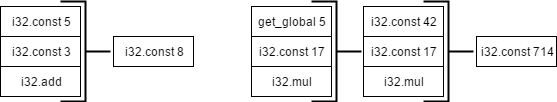
\includegraphics[width=0.65\textwidth]{PeepholeOptimisationIllustrations}
	\centering
	\caption{The applied optimisation to the left stack is simple: adding two constants can be reduced to the result of the addition. The optimisation on the right hand side is more complex: suppose we have a global at position 5 that is immutable and contains the value 42. We can convert the get-call to the value of the variable, as it will never change, which leads to an operation sequence that resembles the one on the left hand side - which, then again, can be can be optimised even further.}
\end{figure}

In a forward compiler, optimising with peephole style optimisations can be added as a pass in the backend compiler, such that when the instruction code is generated, the compiler will run through it again, this time attempting to apply optimisations which attempts to reduce and remove code. For instance, if a function in a program adds two constants together and returns the result, an optimising compiler will reduce the expression to the result of the addition operation, and simply return that: \mintinline{c}{return 7+14; => return 21;}. The logic has not been tampered with, but the function is now 3 operations cheaper\footnote{One for each of the stack reads (reading 7 and 14) and then one for the resulting write operation.}. A more elaborate example can be found below.

\begin{figure}[H]
	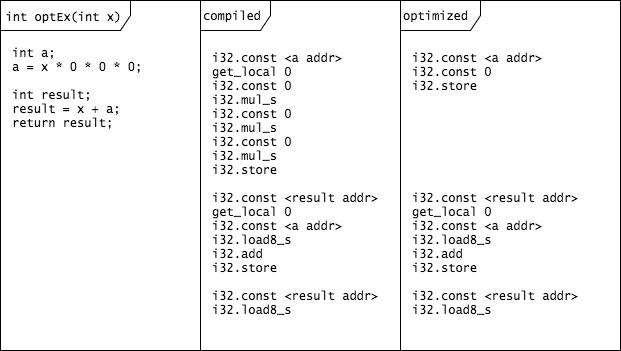
\includegraphics[width=0.75\textwidth]{PeepholeOptimisation}
	\centering
	\caption{A simple function \texttt{optEx} multiplies the input argument with $0$ a few times and then returns the result of an addition. To the right of the function are the compiled and optimised versions of the code in WebAssembly stack machine code.}
\label{fig:peephole-optimisation}
\end{figure}
As can be seen in figure~\ref{fig:peephole-optimisation}, only the multiplication expressions are simplified. While peephole optimising, the compiler will not know if it can discard \texttt{a} entirely, as it could be referenced later, and the compiler does not know the value of \texttt{x}, nor what \texttt{a} contains anymore (we can see that it is equal to $0$, but our brains collect a lot of state regarding the program at hand, which allows us to deduce this), therefore, nothing can be optimised at the end of the function. Running a more complex and stateful optimisation technique could detect more redundant code, but such an optimisation is more resource- and time consuming.

Peephole optimisations fall short when more elaborate optimisations are needed. For instance, if you have many small functions you may want to inline them where used. If we reuse the example from above, with the add function, simply adding the result to the stack rather than calling the function each place is fewer operations, thus inlining would yield a benefit. During peephole optimisation, you won't have information regarding the environment, thus you won’t know what the function that is being called will do, and will not know if inlining is legal.

\section{Conclusion}
\label{sec:conclusion}
% Remember to discuss which things went wrong, and why.

\section{References}
\label{sec:references}
\begingroup
\renewcommand{\section}[2]{}%
\bibliographystyle{plain}
\bibliography{Bibliography}{}
\endgroup

\newpage
\section{Appendix}
\label{sec:appendix}

\subsection{WebAssembly Examples}
\label{sec:appendix:wasm-examples}

\subsubsection{Print module compiled to WASM, explained}
\label{sec:appendix:wasm-examples:binary-print}
\begin{minted}[tabsize=2,breaklines]{text}
; Header
00 61 73 6D                  ; translates to '\0asm', WebAssembly magic number. Exists for quick file type detection.
01 00 00 00                  ; Version number (1)

; Section "Type" (1)
01                           ; Section code: 0x01 = Type
08                           ; Section size: 0x08 bytes (the following 8 bytes are contained within this section)
02                           ; Number of types in section: 2 types
; type 0
60                           ; Type code: 0x60 = function
01                           ; Number of params: 0x01
7F                           ; Type of 1st param: 0x7F = i32
00                           ; Number of results: 0x00
; type 1
60                           ; Type code: 0x60 = function
00                           ; Number of params: 0x00
00                           ; Number of results: 0x00

; Section "Import" (2) - spec: optional
02                           ; Section code: 0x02 = Import
12                           ; Section size: 0x12 bytes (decimal: 18)
01                           ; Number of imports: 0x1
; import header 0
07                           ; String length: 0x07 bytes
69 6D 70 6F 72 74 73         ; Import module name: ascii => "imports"
06                           ; String length: 0x06 bytes
70 72 69 6E 74 69            ; Import field name: ascii => "printi"
00                           ; Import kind: 0x00 (using external_kinds table: 0 = function) "https://github.com/WebAssembly/design/blob/master/BinaryEncoding.md#external_kind"
00                           ; Import signature index: 0x00 (referring to function signature at type 0)

; Section "Function" (3) - spec: required
03                           ; Section code: 0x03 = Function
02                           ; Section size: 0x02 bytes
01                           ; Number of functions: 0x01
01                           ; Function 0 signature index: 0x01 (refers to type 1)

; Section "Start" (8) - spec: optional
08                           ; Section code: 0x08 = Start
01                           ; Section size: 0x01 bytes
01                           ; Start function index (refers to function 1)

; Section "Code" (10) - spec: required
0A                           ; Section code: 0x0a = Code (decimal: 10)
11                           ; Section size: 0x11 bytes (decimal: 17)
01                           ; Number of functions: 0x01
0F                           ; Function body size: 0x0f (decimal: 15)
01                           ; Local variable declaration count: 0x01
01                           ; Local type count of immediate type identifier: 0x01
7F                           ; Type identifier for i32
41                           ; i32.const (the next opcode will be a literal)
05                           ; i32 literal: 0x05
41                           ; i32.const
03                           ; i32 literal: 0x03
6A                           ; i32.add (pop two values from stack, and add them, push result onto stack)
21                           ; set_local, take the next value pushed to the stack, and assign local at that index with stack pop value
00                           ; local variable index: 0x00
20                           ; get_local, take the next value pushed to the stack, and push local at that index onto stack
00                           ; local variable index: 0x00
10                           ; call function at index from next value pushed to stack
00                           ; function index: 0x00
0B                           ; end
\end{minted}

\newpage
\subsection{Code}
\label{sec:appendix:code}
The full source code can be found in the \texttt{.zip}-file that contained this report. If you only have the report in PDF format, see https://github.com/AndreasHassing/microc-to-webassembly.

\subsubsection{micro-wac/pre-build-lexpar-comp.\{sh$|$ps1\}}
\label{sec:appendix:code:pre-build-lexpar-comp}
\textbf{PowerShell Version}
\inputminted[breaklines,tabsize=2,linenos]{powershell}{../micro-wac/pre-build-lexpar-comp.ps1}

\newpage
\noindent\textbf{Bash Version}
\inputminted[breaklines,tabsize=2,linenos]{bash}{../micro-wac/pre-build-lexpar-comp.sh}

\newpage
\subsubsection{micro-wac/WasmBootstrapTemplate.html}
\label{sec:appendix:code:bootstrap-template}
\inputminted[breaklines,tabsize=2,linenos]{html}{../micro-wac/WasmBootstrapTemplate.html}

\newpage
\subsubsection{micro-wac/Wasmcomp.fs}
\label{sec:appendix:code:Wasmcomp.fs}
\inputminted[breaklines,tabsize=2,linenos]{fsharp}{../micro-wac/Wasmcomp.fs}

\newpage
\subsubsection{micro-wac/test/scope.c}
\label{sec:appendix:code:test-scope.c}
\inputminted[breaklines,tabsize=2,linenos]{c}{../micro-wac/test/scope.c}

\newpage
\subsubsection{micro-wac/test/plc/ex2.c}
\label{sec:appendix:code:plc-ex2.c}
\inputminted[breaklines,tabsize=2,linenos]{c}{../micro-wac/test/plc/ex2.c}

\end{document}
